\subsection{Analysis of the recycling of differents thermoplastics for 3D Printing- by Antonio Araujo}

Concerning the first point of only virgin material was considered, Antonio Araujo proposed a methodology that defines in a safe way the technical feasibility of recycling a thermoplastic material for 3D printing, using the extrusion process and the additive manufacturing FDM technology.

As a context for this research, four types of materials from the association Broplast were considered (figure \ref{Context.Antonio})

\begin{figure}[H]
	\centering
	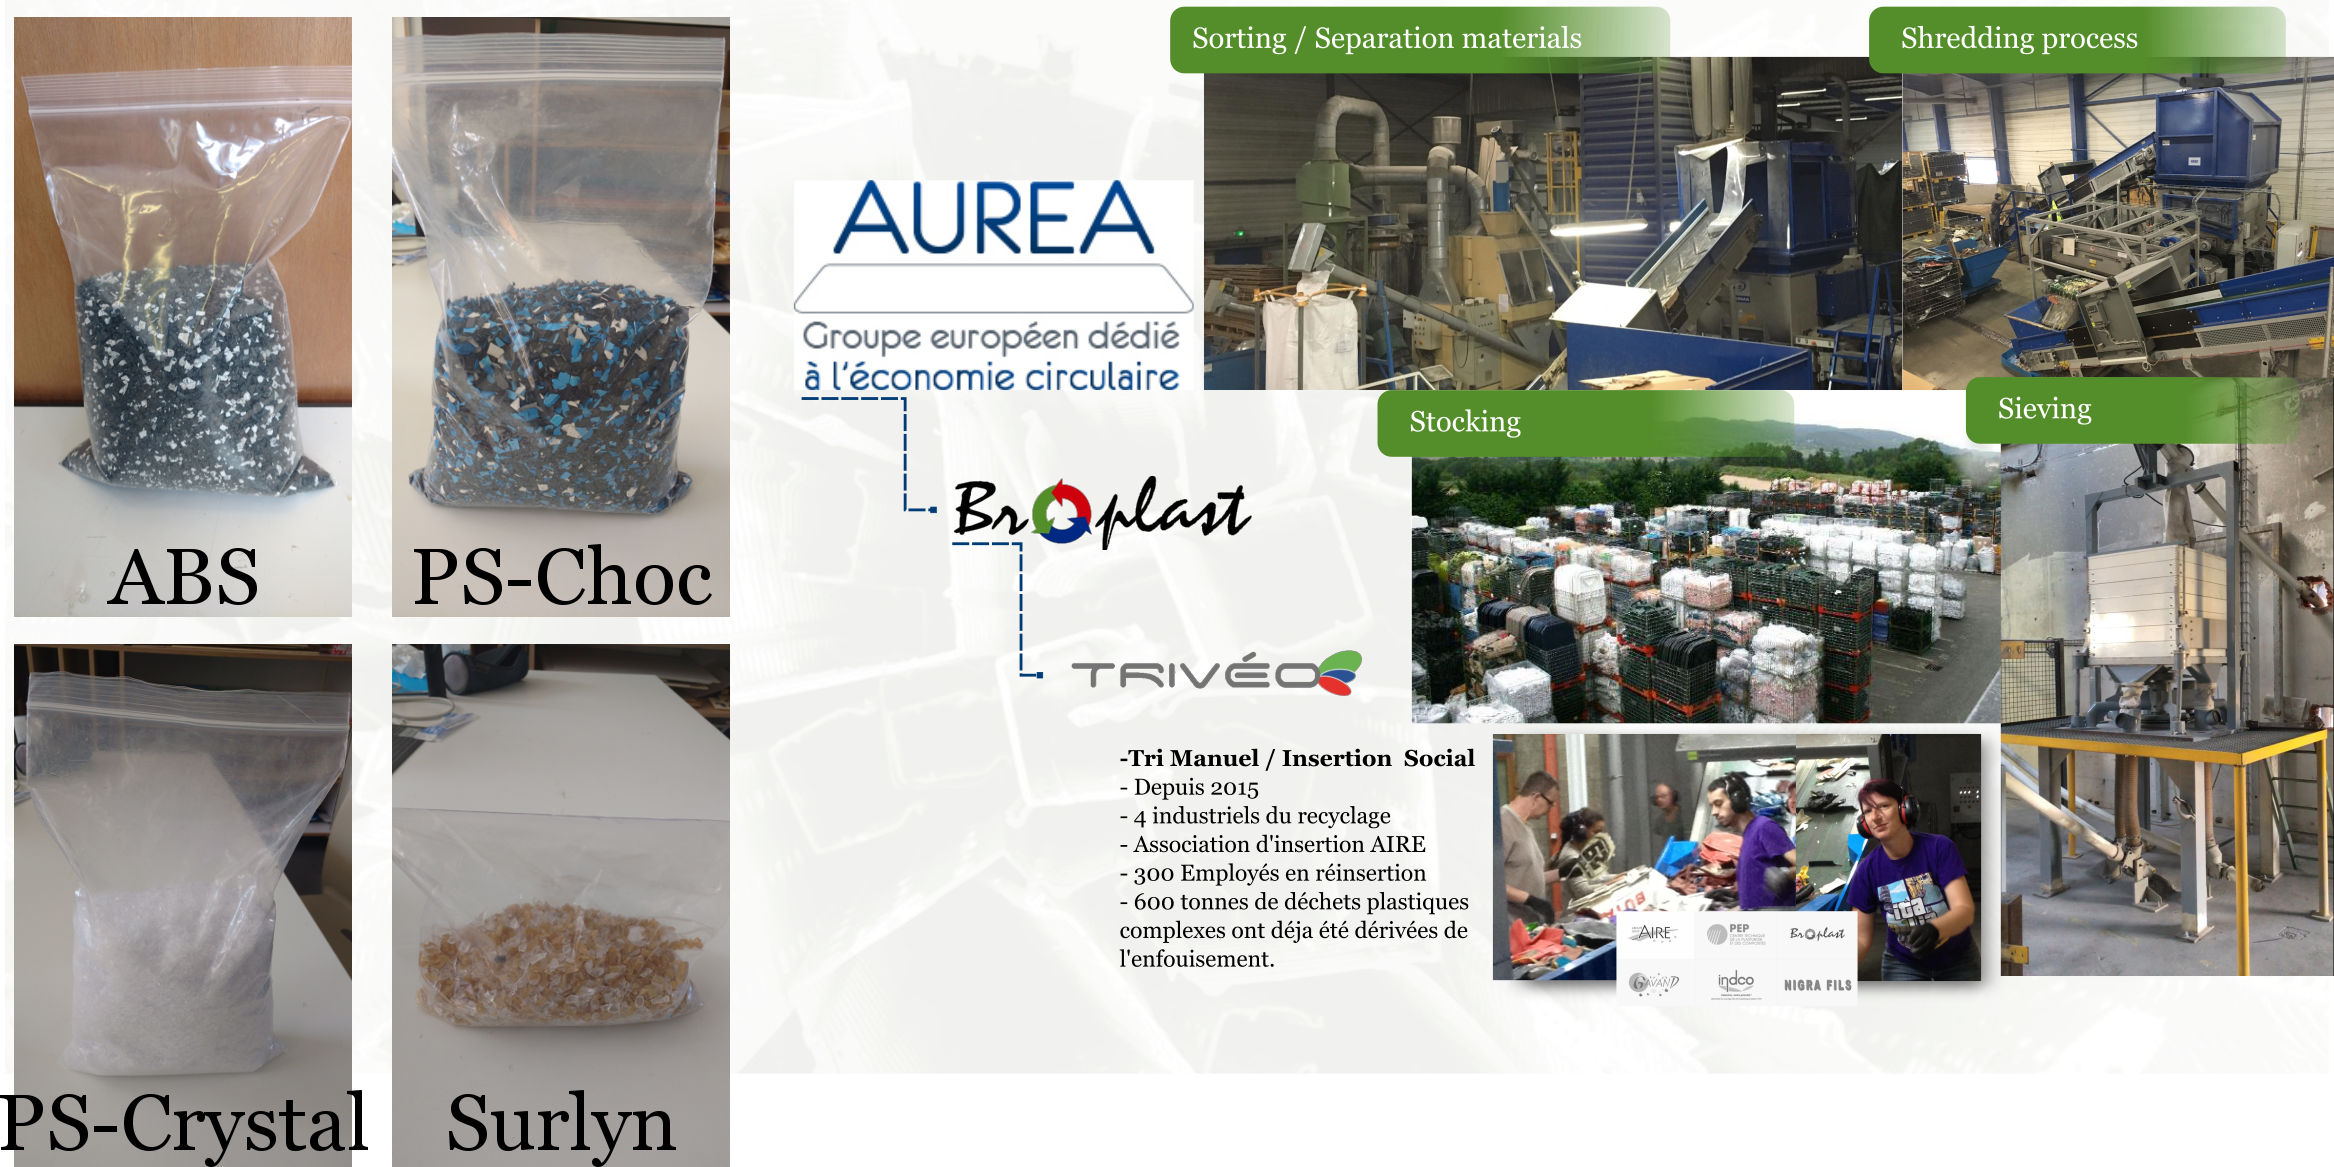
\includegraphics[width=0.8\textwidth]{Figures/Antonio/Context.png}
	\caption{Four materials from Broplast Association}
	\label{Context.Antonio}
\end{figure}


Figure \ref{Methodology.Antonio} shows the proposed methodology.

\begin{figure}[H]
	\centering
	
	\begin{subfigure}{0.55\textwidth}
		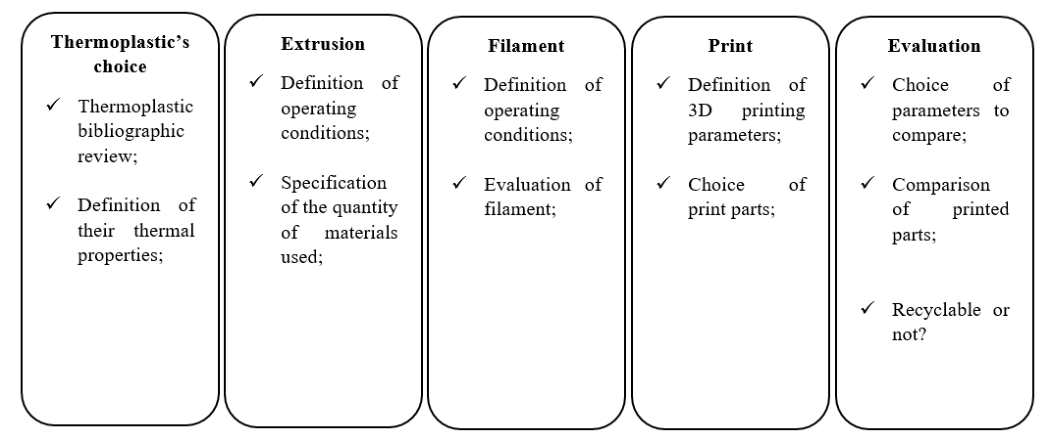
\includegraphics[width=\textwidth]{Figures/Antonio/Methodology.pdf}
		\caption{Methodological framework for recycling in 3DP.}
		\label{Methodology.Antonio}
	\end{subfigure}
	\hfill
	\begin{subfigure}{0.4\textwidth}
		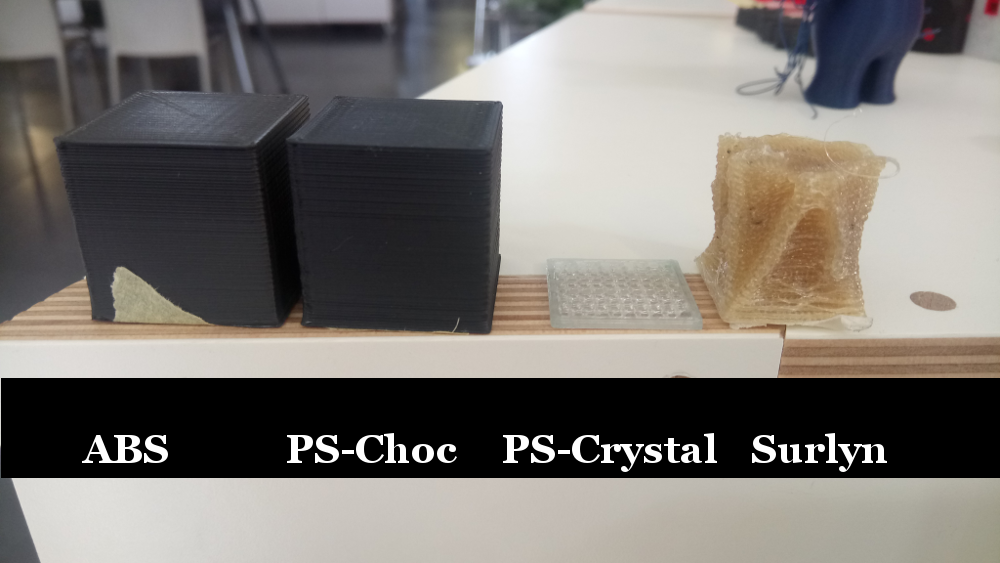
\includegraphics[width=0.8\textwidth]{Figures/Antonio/Final-Results.png} 
		\caption{Operational methodology for recycling in 3DP.}
		\label{Results.Antonio}		
	\end{subfigure}

	
	\caption{Methodology and results for screening aporoach for recycling process}
	\label{Research.Antonio}
\end{figure}